\begin{tikzpicture}
	\draw (0,1) -- (7,2);
	\draw (0,0) -- (7,2) -- (10,-3)  -- cycle; \\[2mm]
\end{tikzpicture} \\[2mm]

\tikz \draw (0,0) rectangle (7,2); \\[2mm]
\tikz \draw (7,0) rectangle (14,-2); \\[2mm]

\begin{tikzpicture}
	\draw (0,0) rectangle (7,2); \\[2mm]
	\draw (7,0) rectangle (14,-2); \\[2mm]
\end{tikzpicture} \\[2mm]

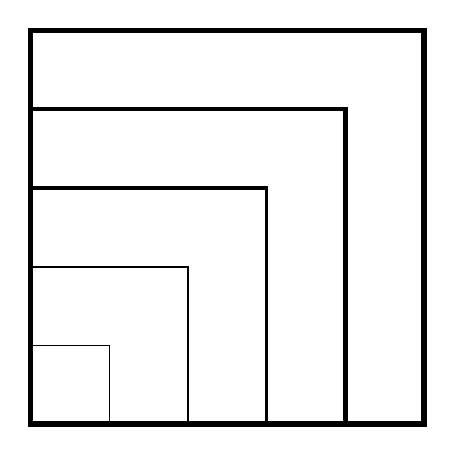
\begin{tikzpicture}
	\draw[thin] (0,0) rectangle (1,1);
	\draw[thick] (0,0) rectangle (2,2);
	\draw[very thick] (0,0) rectangle (3,3);
	\draw[ultra thick] (0,0) rectangle (4,4);  \\[2mm]
	\draw[line width=2pt] (0,0) rectangle (5,5); 
\end{tikzpicture} \\[2mm]

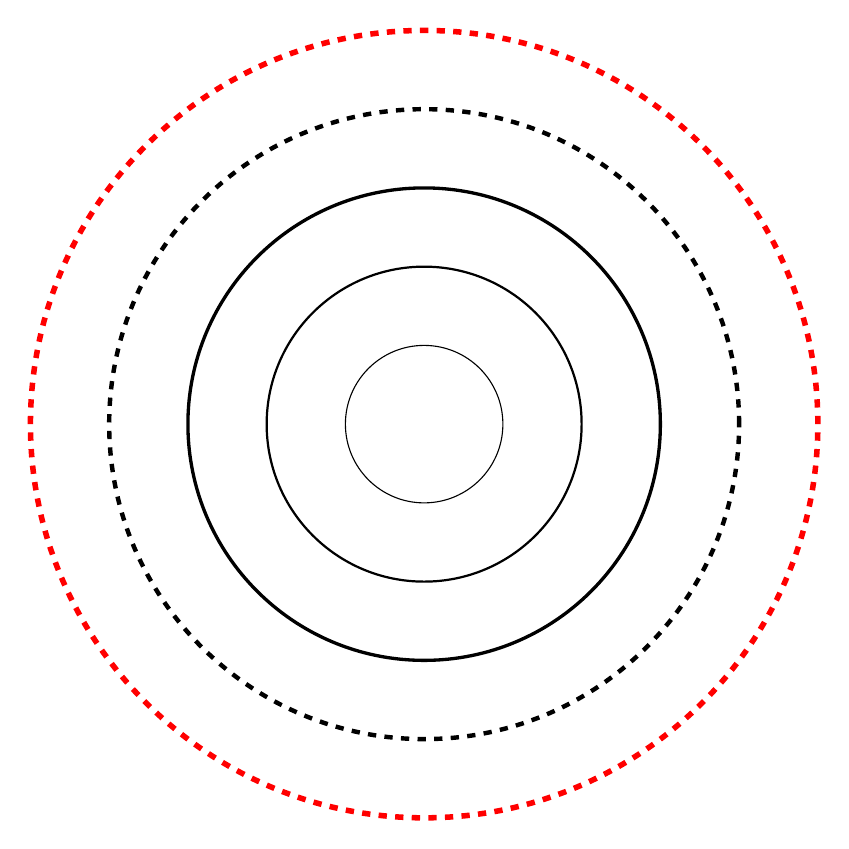
\begin{tikzpicture}
	\draw[thin] (2,2) circle (1);
	\draw[thick] (2,2) circle (2);
	\draw[very thick] (2,2) circle (3);
	\draw[dashed, ultra thick] (2,2) circle (4);
	\draw[dashed, line width=2, color=red] (2,2) circle (5);
\end{tikzpicture} \\[2mm]

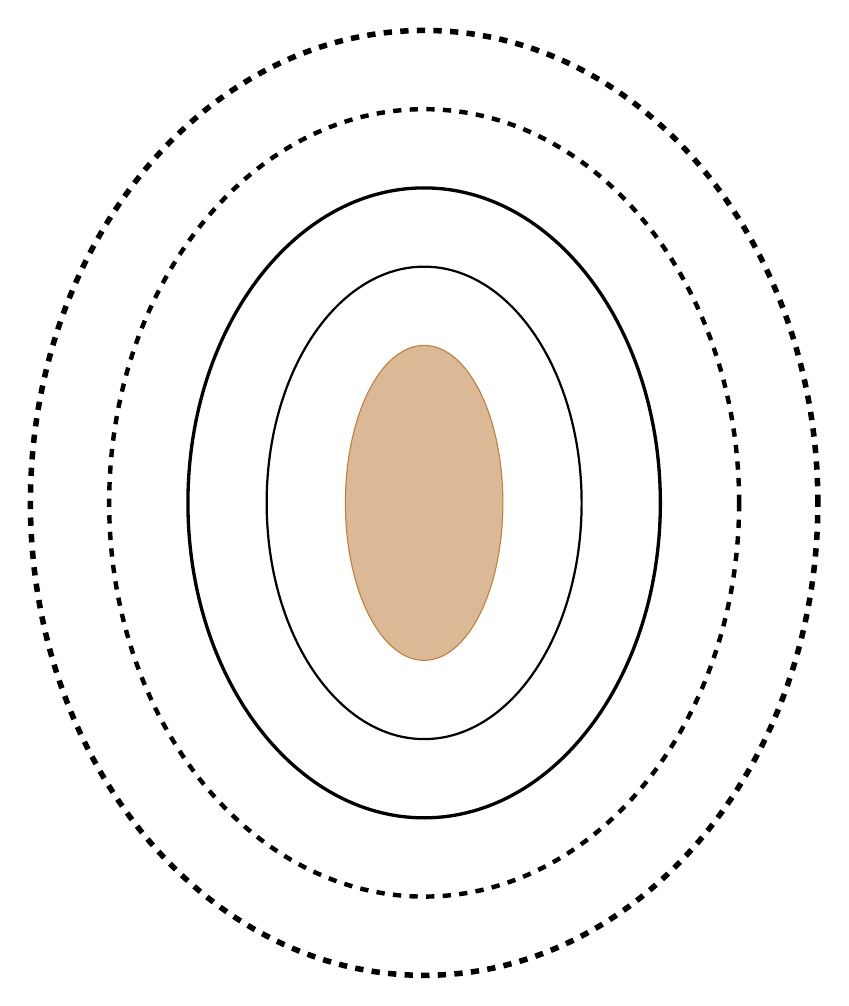
\begin{tikzpicture}
	\draw[thin, color=brown, fill=brown!55] (2,2) ellipse (1 and 2);
	\draw[thick] (2,2) ellipse (2 and 3);
	\draw[very thick] (2,2) ellipse (3 and 4);
	\draw[dashed, ultra thick] (2,2) ellipse (4 and 5);
	\draw[dashed, line width=2pt] (2,2) ellipse (5 and 6);
\end{tikzpicture}  \\[2mm]

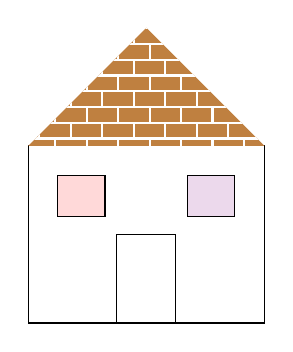
\begin{tikzpicture}[scale=.75]
	\draw (0,0) rectangle (4,3);
	% 1) Fondo marron
	\fill[brown] (0,3) -- (2,5) -- (4,3) -- cycle;
	% 2) Patrón de ladrillos blanco encima
	\pattern[pattern=bricks, pattern color=white]
	(0,3) -- (2,5) -- (4,3) -- cycle;
	\draw (1.5,0) rectangle (2.5,1.5);
	\draw[fill=red!15] (0.5,1.8) rectangle (1.3,2.5);
	\draw[fill=violet!15] (2.7,1.8) rectangle (3.5,2.5);
\end{tikzpicture}  \\[2mm]

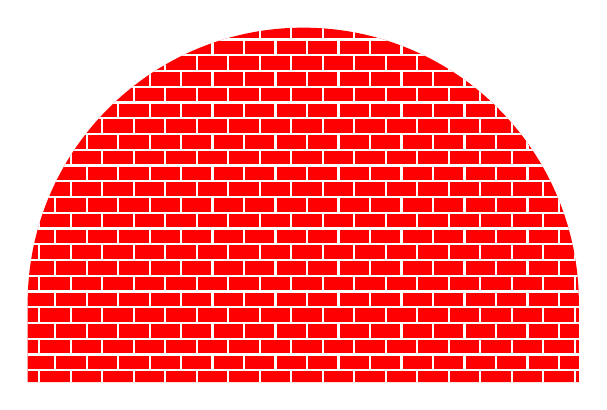
\begin{tikzpicture}
	\def\mypath{(0,0) -- +(0,1) arc (180:0:3.5cm) -- +(0,-1)}
	\fill [red] \mypath;
	\pattern[pattern color=white,pattern=bricks] \mypath;
\end{tikzpicture}  \\[2mm]

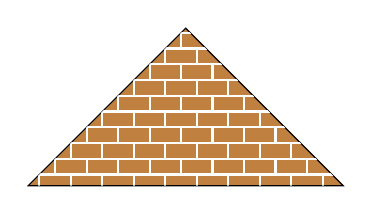
\begin{tikzpicture}
	% 1) Fondo rojo
	\fill[fill=brown, draw=black] (0,3) -- (2,5) -- (4,3) -- cycle;
	% 2) Patrón de ladrillos blanco encima
	\pattern[pattern=bricks, pattern color=white]
	(0,3) -- (2,5) -- (4,3) -- cycle;
\end{tikzpicture}  \\[2mm]

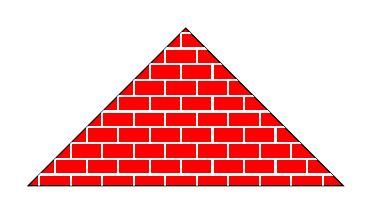
\begin{tikzpicture}
	% 1) Fondo rojo
	\filldraw[fill=red, draw=black]
	(0,3) -- (2,5) -- (4,3) -- cycle;
	\pattern[pattern=bricks, pattern color=white]
	(0,3) -- (2,5) -- (4,3) -- cycle;
\end{tikzpicture}  \\[2mm]

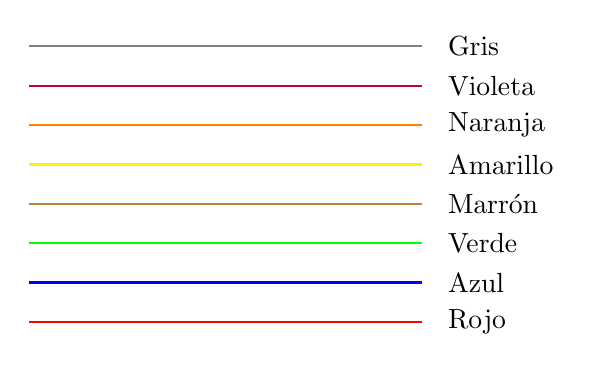
\begin{tikzpicture}
	
	\draw[red, thick] (0,0) -- (5,0); \\[2mm]
	\draw[blue, thick] (0,0.5) -- (5,0.5); \\[2mm]
	\draw[green, thick] (0,1) -- (5,1); \\[2mm]
	\draw[brown, thick] (0,1.5) -- (5,1.5); \\[2mm]
	\draw[yellow, thick] (0,2) -- (5,2); \\[2mm]
	\draw[orange, thick] (0,2.5) -- (5,2.5); \\[2mm]
	\draw[purple, thick] (0,3) -- (5,3); \\[2mm]
	\draw[gray, thick] (0,3.5) -- (5,3.5); \\[2mm]
	
	\node[right] at (5.2,0) {Rojo}; \\[2mm]
	\node[right] at (5.2,0.5) {Azul}; \\[2mm]
	\node[right] at (5.2,1) {Verde}; \\[2mm]
	\node[right] at (5.2,1.5) {Marrón}; \\[2mm]
	\node[right] at (5.2,2) {Amarillo}; \\[2mm]
	\node[right] at (5.2,2.5) {Naranja}; \\[2mm]
	\node[right] at (5.2,3) {Violeta}; \\[2mm]
	\node[right] at (5.2,3.5) {Gris}; \\[2mm]
	
\end{tikzpicture}  \\[2mm]


\begin{tikzpicture}
	\fill[red, pattern=dots] (6,0) rectangle (8,2);
	
	\draw[ultra thin, color=red, opacity=.15, ultra thick, fill=violet, opacity=.15] (0,0) rectangle (3,2) ;  \\[2mm]
	
	\draw[ultra thin, color=red, opacity=.15, ultra thick, fill=violet, opacity=.15] (0,0) rectangle (3,2) ;  
\end{tikzpicture}  \\[2mm]

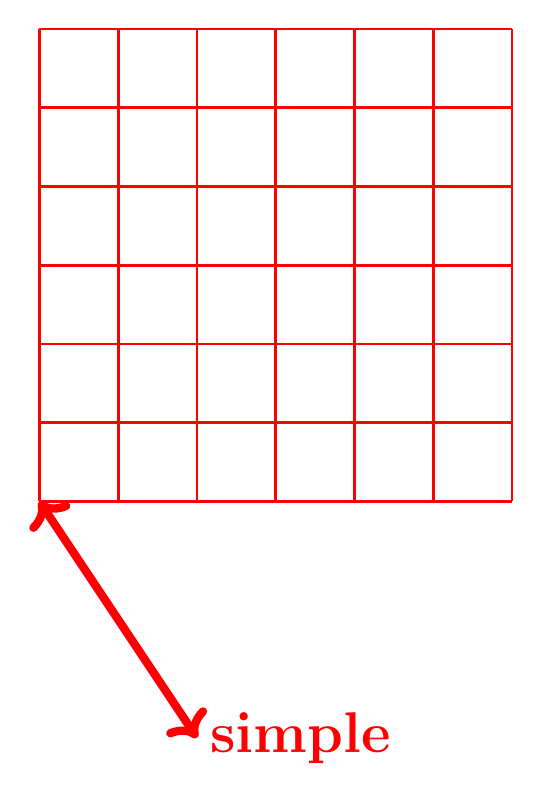
\begin{tikzpicture}
	\draw[red, line width=1] (0,0) grid (6,6); \\[2mm]
	
	\draw[<->, line width=3, red] (0,0) -- (2,-3) node [right] {\huge \textbf{simple}};
\end{tikzpicture}

\begin{tikzpicture}
	%\draw[help lines, gray!30] (-1,-1) grid (4,6);  \\[2mm]
	\draw[gray, thin] (-3,-3) -- (2,-3);  \\[2mm]
	
	\fill[red] (0:2) circle (2pt) node[right] {(0:2)};  \\[2mm]
	
	\foreach \a/\r in {0/2, 45/2, 90/2, 135/2,180/2, 270/2} 
	\draw[violet, dashed] (0,0) -- (\a:\r);  \\[2mm]
	
\end{tikzpicture}  \\[2mm]


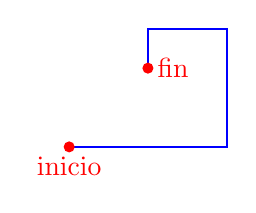
\begin{tikzpicture}
	\draw[thick, blue] (0,0) -- ++(2,0) -- ++(0,1.5) -- ++(-1,0) -- ++(0,-0.5);
	\fill[red] (0,0) circle (2pt) node[below] {inicio};
	\fill[red] (1,1) circle (2pt) node[right] {fin};
\end{tikzpicture}  \\[2mm]


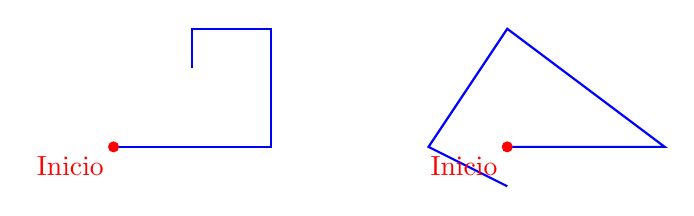
\begin{tikzpicture}[scale=1]
	% Caso con ++
	\draw[thick, blue] (0,0) -- ++(2,0) -- ++(0,1.5) -- ++(-1,0) -- ++(0,-0.5);
	\fill[red] (0,0) circle (2pt) node[below left]{Inicio};
	
	\begin{scope}[xshift=5cm] % separar los dos casos
		% Caso con +
		\draw[thick, blue] (0,0) -- +(2,0) -- +(0,1.5) -- +(-1,0) -- +(0,-0.5);
		\fill[red] (0,0) circle (2pt) node[below left]{Inicio};
	\end{scope}
\end{tikzpicture}  \\[2mm]


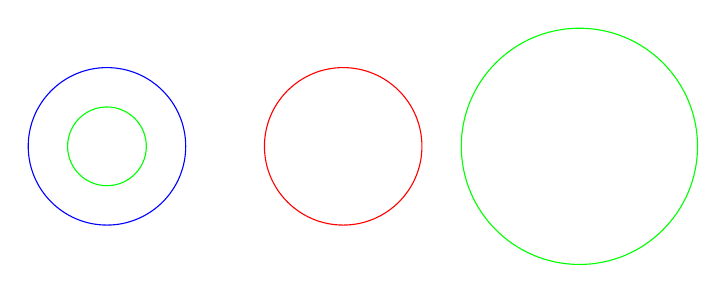
\begin{tikzpicture}
	% Primer círculo en el origen
	\draw[blue] (0,0) circle (1cm);
	
	% Segundo círculo dentro de un scope desplazado
	\begin{scope}[xshift=3cm]
		\draw[red] (0,0) circle (1cm);
	\end{scope}
	
	\begin{scope}[xshift=6cm, scale=3]
		\draw[green] (0,0) circle (0.5cm);
	\end{scope}
	% Tercer círculo (vuelve al origen)
	\begin{scope}[xshift=0cm]
		\draw[green] (0,0) circle (0.5cm);
	\end{scope}
\end{tikzpicture}  \\[2mm]

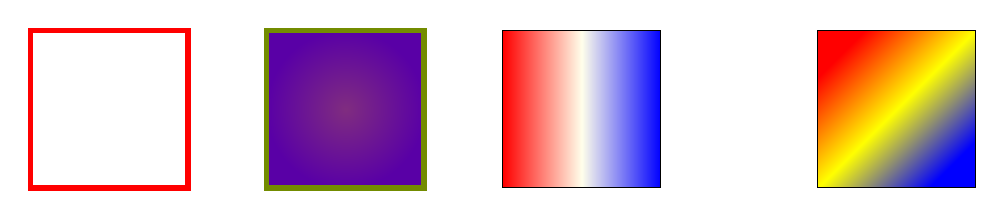
\begin{tikzpicture}
	\draw[draw = red, line width =2pt] (0,0) rectangle (2,2);
	
	\shadedraw[inner color = violet!65!gray, outer color = blue!65!red, red!45!green, line width =2pt] (3,0) rectangle (5,2);
	
	\shadedraw[left color=red, right color=blue, middle color=yellow!8] (6,0) rectangle (8,2);
	
	\shadedraw[left color=red, right color=blue, middle color=yellow, shading angle=45] (10,0) rectangle (12,2);
	
\end{tikzpicture}  \\[2mm]

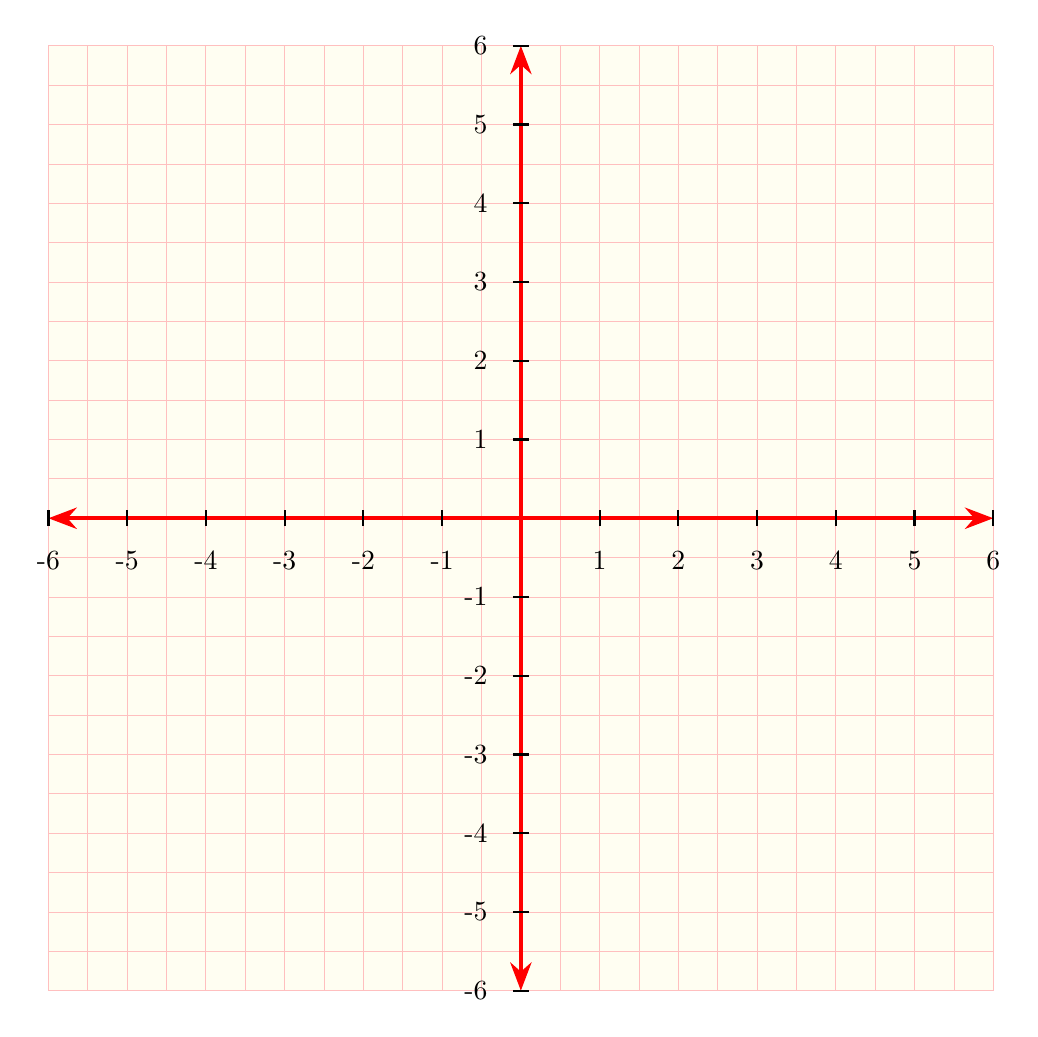
\begin{tikzpicture}
	
	\begin{scope}[on background layer]
		\fill[yellow!5] (-6,-6) rectangle (6,6);
	\end{scope}
	
	\begin{scope}
		\draw[step=.5, draw = red!25, line width =.3pt] (-6,-6) grid (6,6);  
		\draw[<->, >=Stealth, ultra thick, red] (0,-6) -- (0,6) ; 
		\draw[<->, >=Stealth, ultra thick, red] (-6,0) -- (6,0) ;
		
		% Marcas de unidades en el eje X
		\foreach \x in {-6,-5,-4,-3,-2,-1,1,2,3,4,5,6}
		\draw[black, thick] (\x,-0.1) -- (\x,0.1);
		
		% Marcas de unidades en el eje Y  
		\foreach \y in {-6,-5,-4,-3,-2,-1,1,2,3,4,5,6}
		\draw[black, thick] (-0.1,\y) -- (0.1,\y);
		
		% Números en el eje X (sin el 0)
		\foreach \x in {-6,-5,-4,-3,-2,-1,1,2,3,4,5,6}
		\node[black, below] at (\x,-0.3) {\x};
		
		% Números en el eje Y (sin el 0)  
		\foreach \y in {-6,-5,-4,-3,-2,-1,1,2,3,4,5,6}
		\node[black, left] at (-0.3,\y) {\y};
	\end{scope}
	
\end{tikzpicture} \\[2mm]

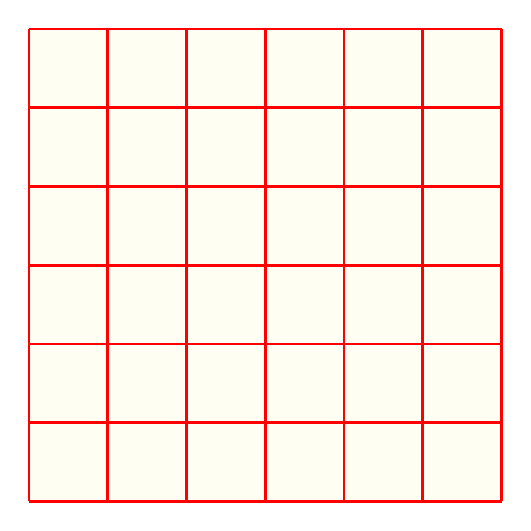
\begin{tikzpicture}
	%\draw[draw = red, line width =2pt] (0,0) rectangle (2,2);
	%\draw[draw = red, line width =2pt, rotate=45] (0,0) rectangle (2,2);
	%\draw[draw = red, line width =2pt, rotate around={45:(2,0)}] (2,0) rectangle (4,2);
	%\draw[draw = red, line width =2pt] (0,0) rectangle (2,2);
	%\draw[draw = red, line width =2pt] (0,0) rectangle (2,2);
	
	% Fondo amarillo del área 0..6 x 0..6
	\fill[yellow!5] (0,0) rectangle (6,6);
	
	% Cuadrícula y flecha por encima del fondo
	\draw[red, line width=1] (0,0) grid (6,6);
	
\end{tikzpicture} \\[2mm]

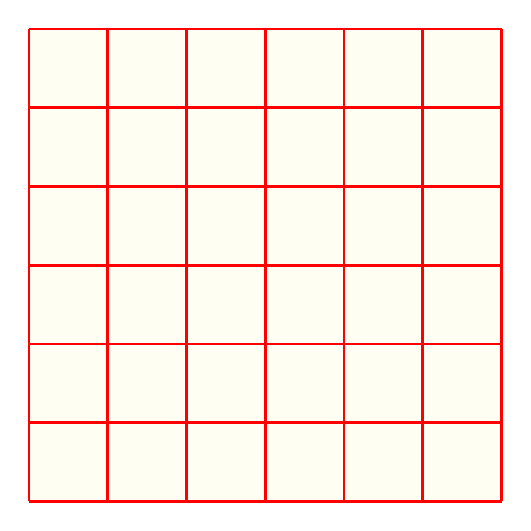
\begin{tikzpicture}
	\begin{scope}[on background layer]
		\fill[yellow!5] (0,0) rectangle (6,6);
	\end{scope}
	
	\draw[red, line width=1] (0,0) grid (6,6);
	
\end{tikzpicture} \\[2mm]

\planoCartesiano{green!5}{violet}{6}{5}

\begin{figure}[H]
	\centering
	\textbf{Experimento: Periodo del Péndulo vs Longitud}
	
	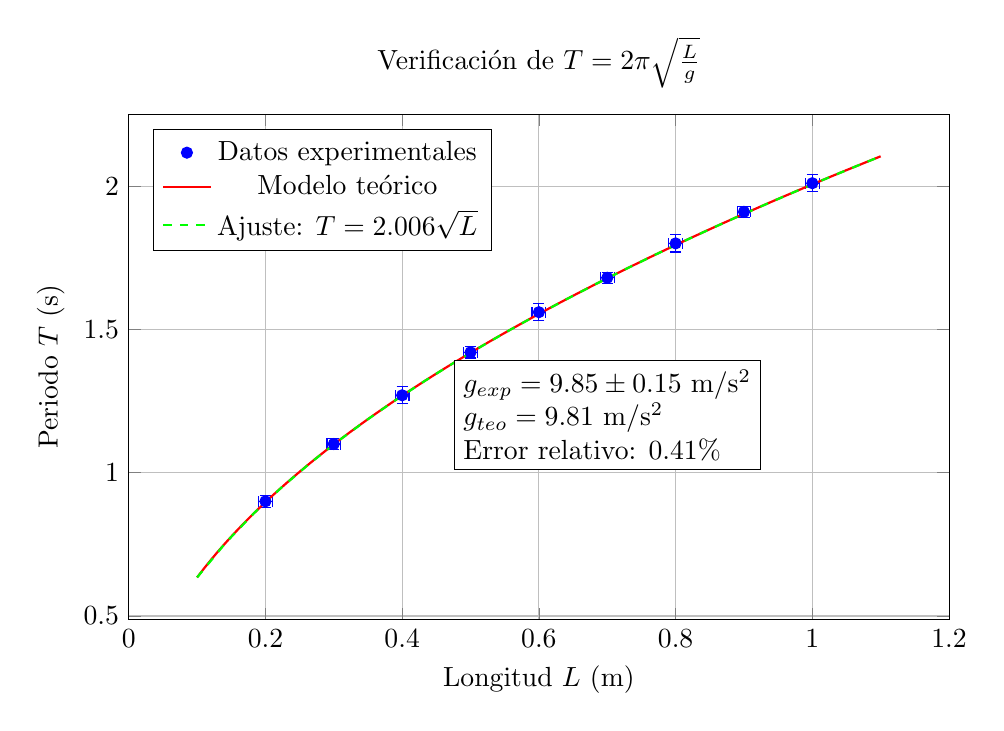
\begin{tikzpicture}
		\begin{axis}[
			title={Verificación de $T = 2\pi\sqrt{\frac{L}{g}}$},
			xlabel={Longitud $L$ (m)},
			ylabel={Periodo $T$ (s)},
			grid=both,
			legend pos=north west,
			width=12cm, height=8cm,
			]
			% Datos experimentales con barras de error
			\addplot[
			only marks, 
			mark=*, 
			mark size=2pt,
			blue,
			error bars/.cd,
			x dir=both, x explicit,
			y dir=both, y explicit,
			] coordinates {
				(0.2,0.90) +- (0.01,0.02)
				(0.3,1.10) +- (0.01,0.02)
				(0.4,1.27) +- (0.01,0.03)
				(0.5,1.42) +- (0.01,0.02)
				(0.6,1.56) +- (0.01,0.03)
				(0.7,1.68) +- (0.01,0.02)
				(0.8,1.80) +- (0.01,0.03)
				(0.9,1.91) +- (0.01,0.02)
				(1.0,2.01) +- (0.01,0.03)
			};
			\addlegendentry{Datos experimentales}
			
			% Modelo teórico
			\addplot[red, thick, domain=0.1:1.1, samples=100] 
			{2*pi*sqrt(x/9.81)};
			\addlegendentry{Modelo teórico}
			
			% Ajuste de curva
			\addplot[green, dashed, thick, domain=0.1:1.1] 
			{2.006*sqrt(x)};
			\addlegendentry{Ajuste: $T = 2.006\sqrt{L}$}
			
			% Información adicional
			\node[fill=white, draw, align=left] at (axis cs:0.7,1.2) {
				$g_{exp} = 9.85 \pm 0.15$ m/s$^2$\\
				$g_{teo} = 9.81$ m/s$^2$\\
				Error relativo: 0.41\%
			};
		\end{axis}
	\end{tikzpicture}
	
	\caption{Comparación entre valores experimentales y teóricos}
\end{figure}

\begin{tikzpicture}
	\begin{groupplot}[
		group style={
			group size=1 by 2,
			vertical sep=1.5cm
		},
		width=12cm, height=5cm,
		grid=both,
		xlabel={Tiempo (s)},
		]
		
		% Gráfica superior: Posición vs tiempo
		\nextgroupplot[
		title={Oscilación Amortiguada},
		ylabel={Posición (cm)},
		]
		% Datos experimentales
		\addplot[blue, mark=*, mark size=0.5pt] table {
			t       x
			0.0     10.0
			0.1     8.5
			0.2     -6.8
			0.3     -7.2
			0.4     6.1
			0.5     5.8
			% ... más datos
		};
		
		% Modelo ajustado
		\addplot[red, thick, domain=0:3, samples=200] 
		{10*exp(-0.5*x)*cos(deg(2*pi*x))};
		
		% Envolvente
		\addplot[green, dashed, domain=0:3] {10*exp(-0.5*x)};
		\addplot[green, dashed, domain=0:3] {-10*exp(-0.5*x)};
		
		% Gráfica inferior: Energía vs tiempo
		\nextgroupplot[
		title={Energía del Sistema},
		ylabel={Energía (mJ)},
		legend pos=north east,
		]
		% Energía cinética
		\addplot[blue, thick, domain=0:3, samples=200] 
		{50*exp(-x)*sin(deg(2*pi*x))^2};
		\addlegendentry{E. Cinética}
		
		% Energía potencial
		\addplot[red, thick, domain=0:3, samples=200] 
		{50*exp(-x)*cos(deg(2*pi*x))^2};
		\addlegendentry{E. Potencial}
		
		% Energía total
		\addplot[black, ultra thick, domain=0:3] 
		{50*exp(-x)};
		\addlegendentry{E. Total}
	\end{groupplot}
\end{tikzpicture}

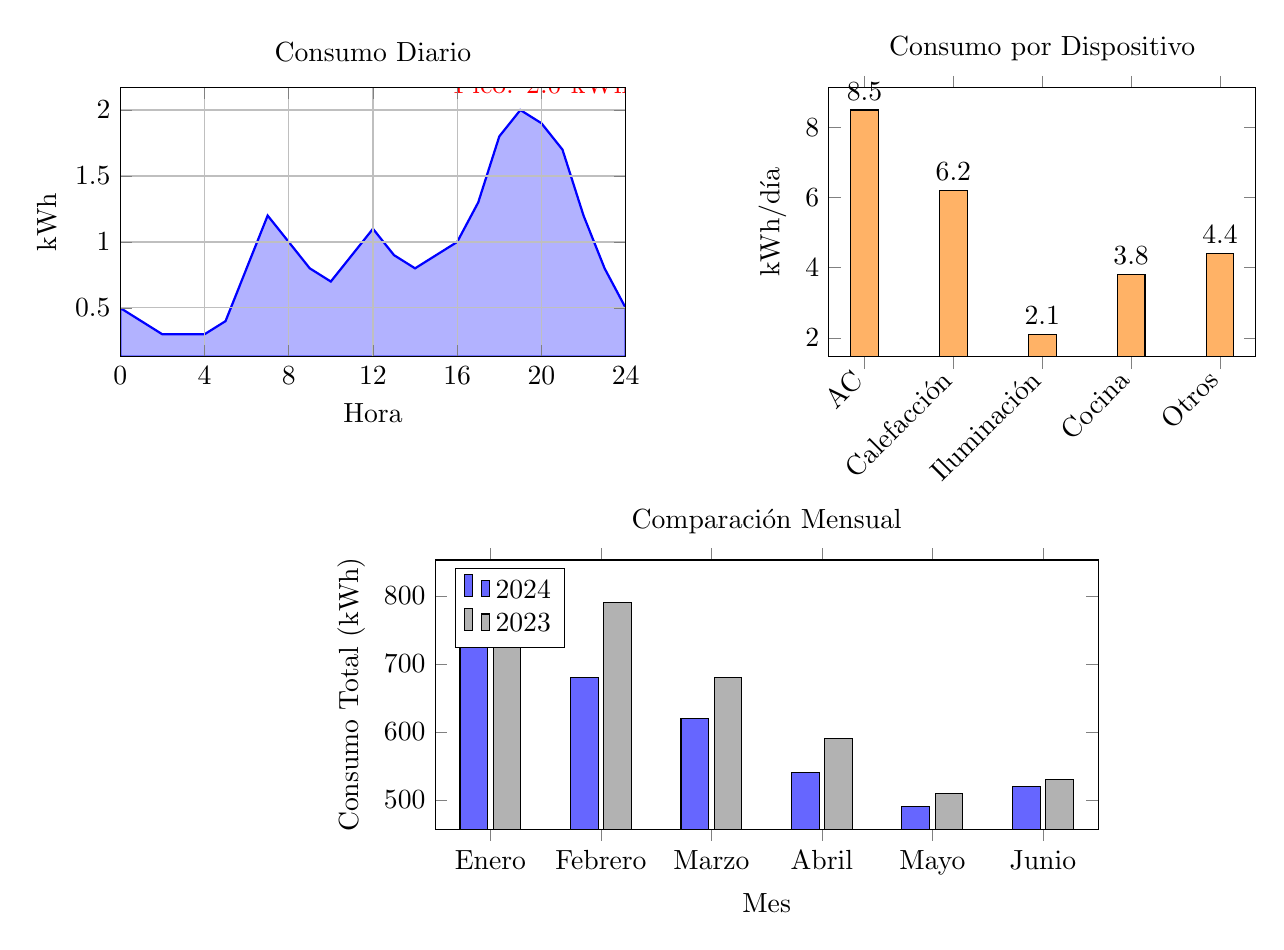
\begin{tikzpicture}
	% Panel 1: Consumo diario
	\begin{axis}[
		at={(0,0)},
		width=8cm, height=5cm,
		title={Consumo Diario},
		xlabel={Hora},
		ylabel={kWh},
		xmin=0, xmax=24,
		xtick={0,4,8,12,16,20,24},
		grid=both,
		area style,
		]
		
		\addplot[fill=blue!30, draw=blue, thick] coordinates {
			(0,0.5) (1,0.4) (2,0.3) (3,0.3) (4,0.3) (5,0.4)
			(6,0.8) (7,1.2) (8,1.0) (9,0.8) (10,0.7) (11,0.9)
			(12,1.1) (13,0.9) (14,0.8) (15,0.9) (16,1.0) (17,1.3)
			(18,1.8) (19,2.0) (20,1.9) (21,1.7) (22,1.2) (23,0.8)
			(24,0.5)
		} \closedcycle;
		
		% Pico de consumo
		\node[red] at (axis cs:20,2.2) {Pico: 2.0 kWh};
	\end{axis}
	
	% Panel 2: Distribución por dispositivo
	\begin{axis}[
		at={(9cm,0)},
		width=7cm, height=5cm,
		title={Consumo por Dispositivo},
		ybar,
		symbolic x coords={AC,Calefacción,Iluminación,Cocina,Otros},
		xtick=data,
		x tick label style={rotate=45, anchor=east},
		ylabel={kWh/día},
		nodes near coords,
		]
		
		\addplot[fill=orange!60] coordinates {
			(AC,8.5) (Calefacción,6.2) (Iluminación,2.1)
			(Cocina,3.8) (Otros,4.4)
		};
	\end{axis}
	
	% Panel 3: Comparación mensual
	\begin{axis}[
		at={(4cm,-6cm)},
		width=10cm, height=5cm,
		title={Comparación Mensual},
		xlabel={Mes},
		ylabel={Consumo Total (kWh)},
		xtick={1,2,3,4,5,6},
		xticklabels={Enero,Febrero,Marzo,Abril,Mayo,Junio},
		ybar,
		legend pos=north west,
		]
		
		\addplot[fill=blue!60] coordinates {
			(1,750) (2,680) (3,620) (4,540) (5,490) (6,520)
		};
		\addlegendentry{2024}
		
		\addplot[fill=gray!60] coordinates {
			(1,820) (2,790) (3,680) (4,590) (5,510) (6,530)
		};
		\addlegendentry{2023}
	\end{axis}
\end{tikzpicture}

\begin{figure}[H]
	\centering
	\textbf{KPI Dashboard - Q4 2024}
	
	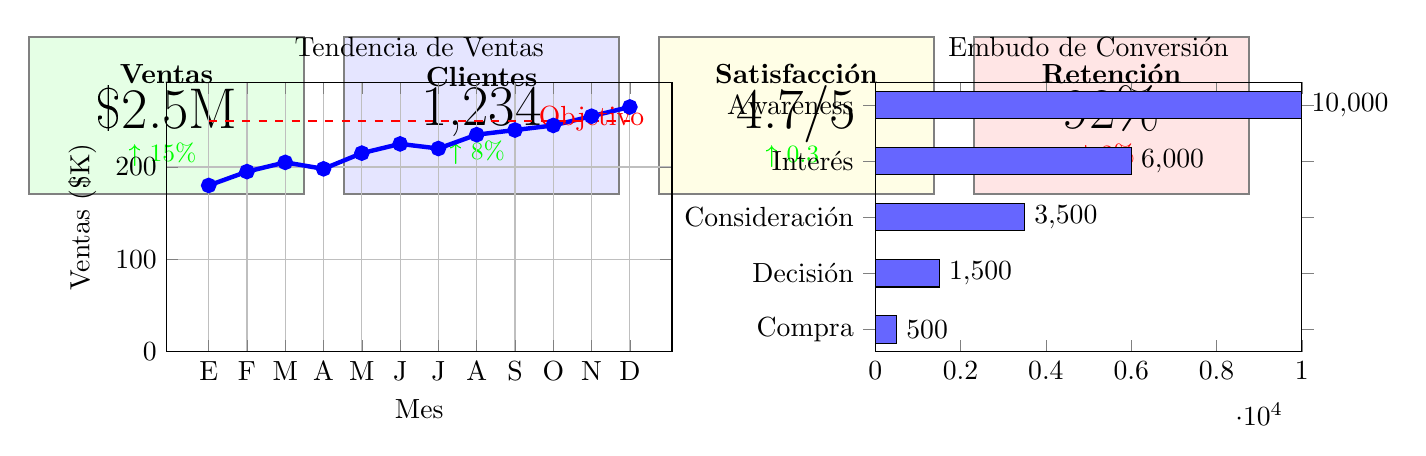
\begin{tikzpicture}
		% Definir estilos corporativos
		\tikzset{
			kpi box/.style={
				draw=gray, 
				thick, 
				fill=white, 
				minimum width=3.5cm, 
				minimum height=2cm,
				align=center
			}
		}
		
		% KPIs principales
		\node[kpi box, fill=green!10] at (0,0) {
			\textbf{Ventas}\\
			\huge\$2.5M\\
			\small\color{green}↑ 15\%
		};
		
		\node[kpi box, fill=blue!10] at (4,0) {
			\textbf{Clientes}\\
			\huge 1,234\\
			\small\color{green}↑ 8\%
		};
		
		\node[kpi box, fill=yellow!10] at (8,0) {
			\textbf{Satisfacción}\\
			\huge 4.7/5\\
			\small\color{green}↑ 0.3
		};
		
		\node[kpi box, fill=red!10] at (12,0) {
			\textbf{Retención}\\
			\huge 92\%\\
			\small\color{red}↓ 2\%
		};
		
		% Gráfico de tendencia
		\begin{axis}[
			at={(0,-3cm)},
			width=8cm, height=5cm,
			title={Tendencia de Ventas},
			xlabel={Mes},
			ylabel={Ventas (\$K)},
			xtick={1,2,3,4,5,6,7,8,9,10,11,12},
			xticklabels={E,F,M,A,M,J,J,A,S,O,N,D},
			grid=both,
			ymin=0,
			]
			
			\addplot[blue, ultra thick, mark=*] coordinates {
				(1,180) (2,195) (3,205) (4,198) (5,215)
				(6,225) (7,220) (8,235) (9,240) (10,245)
				(11,255) (12,265)
			};
			
			% Objetivo
			\addplot[red, dashed, thick, domain=1:12] {250};
			\node[red] at (axis cs:11,252) {Objetivo};
		\end{axis}
		
		% Embudo de ventas
		\begin{axis}[
			at={(9cm,-3cm)},
			width=7cm, height=5cm,
			title={Embudo de Conversión},
			xbar,
			symbolic y coords={Compra,Decisión,Consideración,Interés,Awareness},
			ytick=data,
			xmin=0, xmax=10000,
			nodes near coords,
			]
			
			\addplot[fill=blue!60] coordinates {
				(10000,Awareness)
				(6000,Interés)
				(3500,Consideración)
				(1500,Decisión)
				(500,Compra)
			};
		\end{axis}
	\end{tikzpicture}
\end{figure}

\begin{center}
	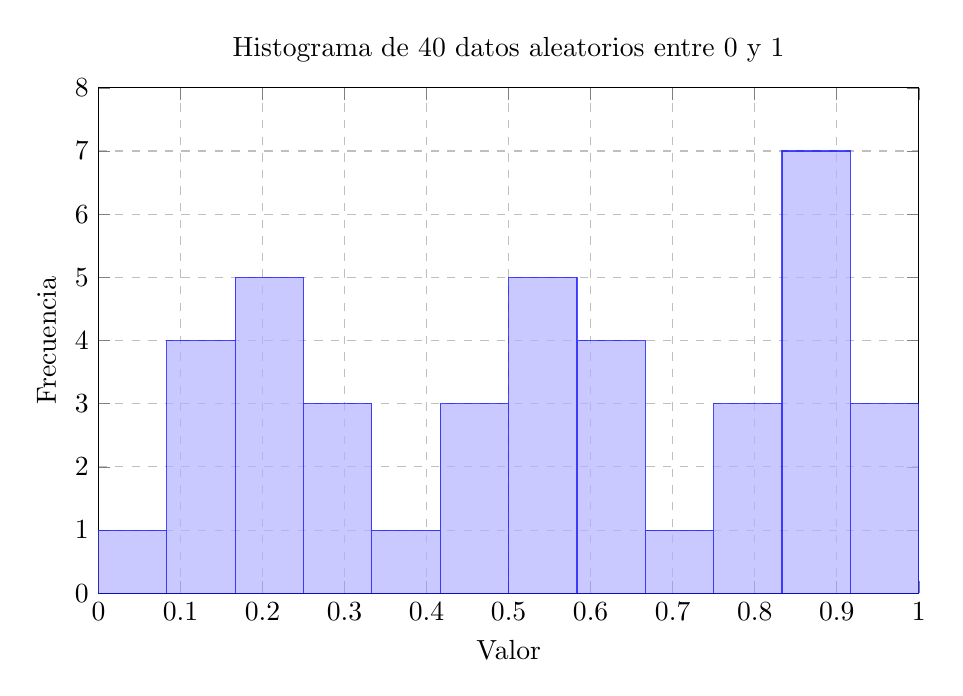
\begin{tikzpicture}
		\begin{axis}[
			width=12cm,
			height=8cm,
			xlabel={Valor},
			ylabel={Frecuencia},
			title={Histograma de 40 datos aleatorios entre 0 y 1},
			xmin=0, xmax=1,
			ymin=0, ymax=8,
			xtick={0,0.1,0.2,0.3,0.4,0.5,0.6,0.7,0.8,0.9,1.0},
			ytick={0,1,2,3,4,5,6,7,8},
			grid=major,
			grid style={dashed},
			]
			
			% Datos aleatorios de ejemplo (40 valores entre 0 y 1) - formato horizontal
			\pgfplotstableread[row sep=\\]{
				0.123\\0.456\\0.789\\0.234\\0.567\\0.890\\0.345\\0.678\\0.012\\0.901\\0.432\\0.765\\0.098\\0.321\\0.654\\0.987\\0.210\\0.543\\0.876\\0.109\\0.642\\0.975\\0.308\\0.631\\0.864\\0.197\\0.520\\0.853\\0.186\\0.419\\0.752\\0.085\\0.618\\0.951\\0.284\\0.517\\0.840\\0.173\\0.506\\0.839\\
			}\datatable
			
			\addplot[
			hist={
				bins=12,
				data min=0,
				data max=1
			},
			fill=blue!30,
			draw=blue,
			opacity=0.7
			] table[y index=0] {\datatable};
			
		\end{axis}
	\end{tikzpicture}
\end{center}




\begin{center}
	\begin{tikzpicture}
		\begin{axis}[
			title={Estructura de Doble Hélice},
			view={45}{30}, 
			width=12cm, 
			height=10cm,
			xlabel={X}, 
			ylabel={Y}, 
			zlabel={Z},
			legend pos=outer north east,
			grid=major,
			axis lines=center,
			xmin=-2, xmax=2,
			ymin=-2, ymax=2,
			zmin=0, zmax=10,
			]
			
			% Primera hebra (azul)
			\addplot3[blue, thick, domain=0:6*pi, samples=200]
			({1.5*cos(deg(x))}, {1.5*sin(deg(x))}, {x/2});
			\addlegendentry{Hebra 1}
			
			% Segunda hebra (roja) - desfasada 180 grados
			\addplot3[red, thick, domain=0:6*pi, samples=200]
			({1.5*cos(deg(x+pi))}, {1.5*sin(deg(x+pi))}, {x/2});
			\addlegendentry{Hebra 2}
			
			% Conexiones transversales (pares de bases)
			\foreach \t in {0.5, 1.0, 1.5, 2.0, 2.5, 3.0, 3.5, 4.0, 4.5, 5.0, 5.5, 6.0, 6.5, 7.0, 7.5, 8.0, 8.5, 9.0, 9.5, 10.0, 10.5, 11.0, 11.5, 12.0, 12.5, 13.0, 13.5, 14.0, 14.5, 15.0, 15.5, 16.0, 16.5, 17.0, 17.5, 18.0}
			{
				\addplot3[gray, thin] coordinates {
					({1.5*cos(deg(\t))}, {1.5*sin(deg(\t))}, {\t/2})
					({1.5*cos(deg(\t+pi))}, {1.5*sin(deg(\t+pi))}, {\t/2})
				};
			}
			
		\end{axis}
	\end{tikzpicture}
\end{center}

\vspace{1cm}

\textbf{Características de la estructura:}
\begin{itemize}
	\item Dos hebras helicoidales entrelazadas
	\item Desfase de 180° entre las hebras
	\item Conexiones transversales simulando pares de bases
	\item Radio de 1.5 unidades
	\item Paso helicoidal proporcional a la altura
\end{itemize}





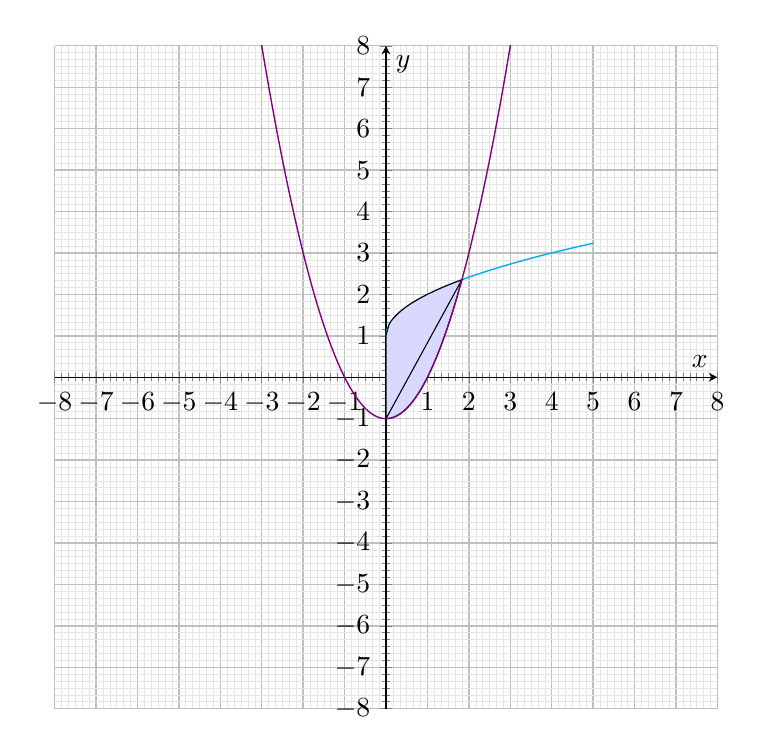
\begin{tikzpicture}
	\begin{axis}[
		width=10cm,
		height=10cm,
		xmin=-8,
		xmax=8,
		ymin=-8,
		ymax=8,
		grid=both,                                 % mayor + menor
		major grid style={line width=.5pt, draw=gray!50},
		minor grid style={line width=.2pt, draw=gray!20},
		xtick distance=1, ytick distance=1,        % separación entre grids mayores
		minor x tick num=5, minor y tick num=5,    % subdivisiones entre marcas mayores
		xlabel=$x$,
		ylabel=$y$,
		xlabel style={at={(ticlabel* cs:1.05)}},
		ylabel style={at={(ticlabel* cs:1.05)}},
		axis x line=center,
		axis y line=center,
		]
		\addplot[cyan,  line width=.5pt,samples=200,domain=0:5] {1+sqrt(x)} ;
		
		
		\filldraw[fill=blue!15] (0,-1) -- plot [smooth, domain=0:1.83] (\x,{1+sqrt(\x)}) -- plot [smooth, domain=0:1.83] (\x, {(\x)^2-1}) ;
		
		
		\addplot[violet, line width=.5pt,samples=200,domain=-5:5] {-1+x^2} ;
	\end{axis}
\end{tikzpicture}



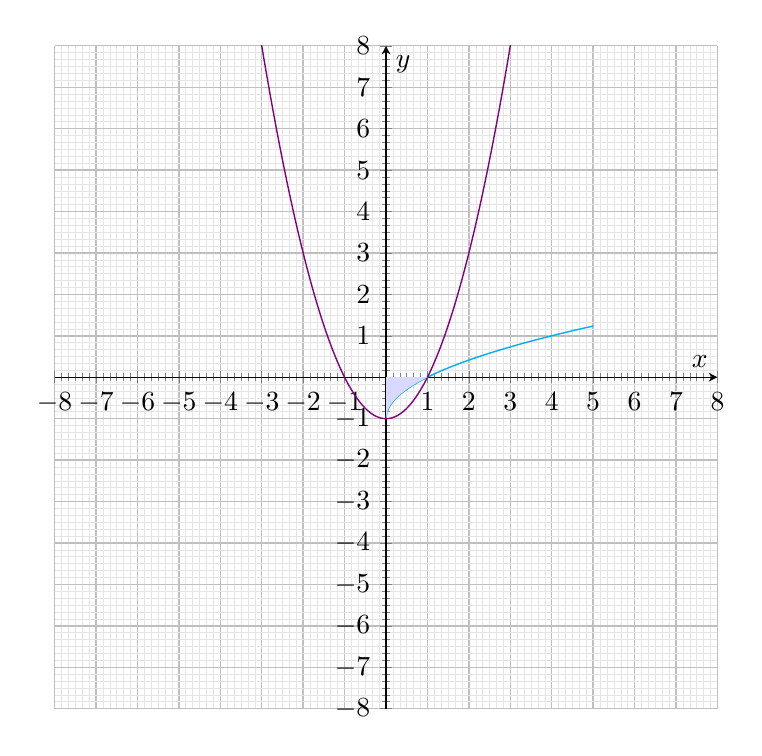
\begin{tikzpicture}
	\begin{axis}[
		width=10cm,
		height=10cm,
		xmin=-8,
		xmax=8,
		ymin=-8,
		ymax=8,
		grid=both,                                 % mayor + menor
		major grid style={line width=.5pt, draw=gray!50},
		minor grid style={line width=.2pt, draw=gray!20},
		xtick distance=1, ytick distance=1,        % separación entre grids mayores
		minor x tick num=5, minor y tick num=5,    % subdivisiones entre marcas mayores
		xlabel=$x$,
		ylabel=$y$,
		xlabel style={at={(ticklabel* cs:1.05)}},  % Corregido: ticklabel en lugar de ticlabel
		ylabel style={at={(ticklabel* cs:1.05)}},  % Corregido: ticklabel en lugar de ticlabel
		axis x line=center,
		axis y line=center,
		]
		
		% Primera función: f(x) = -1 + sqrt(x) (dominio x >= 0)
		\addplot[cyan, line width=.5pt, samples=200, domain=0:5] {-1+sqrt(x)};
		
		% Segunda función: g(x) = -1 + x^2
		\addplot[violet, line width=.5pt, samples=200, domain=-5:5] {-1+x^2};
		
		% Área entre las curvas (si es lo que se busca)
		% Nota: El área original tenía errores en la definición
		\addplot[fill=blue!15, draw=none, domain=0:1] {-1+sqrt(x)} \closedcycle;
		
	\end{axis}
\end{tikzpicture}  \\[5mm]

\begin{tikzpicture}
	\begin{axis}[
		width=10cm, height=10cm,
		xmin=-8, xmax=8, ymin=-8, ymax=8,
		grid=both,
		major grid style={line width=.5pt, draw=gray!50},
		minor grid style={line width=.2pt, draw=gray!20},
		xtick distance=1, ytick distance=1,
		minor x tick num=5, minor y tick num=5,
		axis x line=center, axis y line=center,
		xlabel={$x$}, ylabel={$y$},
		xlabel style={at={(axis description cs:1.05,0)}, anchor=west},
		ylabel style={at={(axis description cs:0,1.05)}, anchor=south},
		]
		% Curvas y nombres de camino
		\addplot[name path=upper, cyan,  line width=.5pt, samples=200, domain=0:5] {1 + sqrt(x)};
		\addplot[name path=lower, violet,line width=.5pt, samples=200, domain=-5:5] {-2 + x^2};
		
		% Área entre curvas en [0, 1.83]
		%\addplot[blue!15] fill between[
		%of=upper and lower,
		%soft clip={domain=0:2.11}
		];
	\end{axis}
\end{tikzpicture}  \\[5mm]


\begin{tikzpicture}
	\begin{axis}[
		width=11cm, height=8cm,
		xmin=0, xmax=4,
		ymin=-2, ymax=4,
		grid=both,
		axis x line=center, axis y line=center,
		xlabel={$x$}, ylabel={$y$},
		legend pos=south east
		]
		
		% Curvas
		\addplot[name path=Funo,  cyan!70!black, very thick, domain=0:4, samples=400] {1 + sqrt(x)};
		\addlegendentry{$f(x)=1+\sqrt{x}$}
		
		\addplot[name path=Fdos,  violet!80!black, very thick, domain=0:4, samples=400] {x^2 - 1};
		\addlegendentry{$g(x)=x^2-1$}
		
		% Punto de cruce aproximado (solución de 1+sqrt(x)=x^2-1)
		% t^4 - t - 2 = 0 con t=sqrt(x) -> x \approx 1.83
		\addplot[densely dashed, violet] coordinates {(1.83,-2) (1.83,4)};
		\node[gray!60, anchor=south west] at (axis cs:1.83, -1.9) {$x\approx 1.83$};
		
		% Área donde f(x) está por ENCIMA de g(x): [0, 1.83]
		\addplot[fill=green!25, draw=none]
		fill between[
		of=Funo and Fdos,
		soft clip={domain=0:1.83}
		];
		
		% Área donde g(x) está por ENCIMA de f(x): (1.83, 4]
		\addplot[fill=orange!25, draw=none]
		fill between[
		of=Fdos and Funo,
		soft clip={domain=1.83:4}
		];
	\end{axis}
\end{tikzpicture}  \\[5mm]

En el intervalo **$[0,\,1.83]$** (verde), \(f(x)=1+\sqrt{x}\) está **por encima** de \(g(x)=x^2-1\).  
A partir de **$x>1.83$** (naranja), las posiciones se **invierten** y \(g(x)\) queda **por encima** de \(f(x)\).  
`fill between` rellena el área **entre dos caminos** nombrados:  
- `of=Funo and Fdos` indica entre cuáles curvas.  
- `soft clip={domain=a:b}` limita el relleno al subintervalo de \(x\) indicado, calculando cortes suaves en los bordes.  \\[25mm]

\begin{tikzpicture}[->]
	\draw (0,0,0) -- (xyz cylindrical cs:radius=1);
	\draw (0,0,0) -- (xyz cylindrical cs:radius=1,angle=90);
	\draw (0,0,0) -- (xyz cylindrical cs:z=1);
\end{tikzpicture} 

% En el cuerpo:
\begin{verbatim}
	Notas rápidas sobre dirtree
	En el cuerpo: 
	Cada línea del árbol termina con un punto (.).
	El número .1, .2, .3, … indica el nivel (raíz = .1).
	El sufijo / tras un nombre indica directorio (muestra la “ramita” abierta).
	Puedes incluir extensiones (.tex, .csv, …) y comentarios como (gráficas generadas) sin problema.
\end{verbatim}

\dirtree{%
	.1 mi-proyecto/.
	.2 main.tex.
	.2 datos/.
	.3 ventas.csv.
	.3 temperaturas.txt.
	.3 experimento.dat.
	.2 figuras/.
	.3 (gráficas generadas).
	.2 codigo/.
	.3 procesamiento.py.
}

\newpage
\begin{center}
	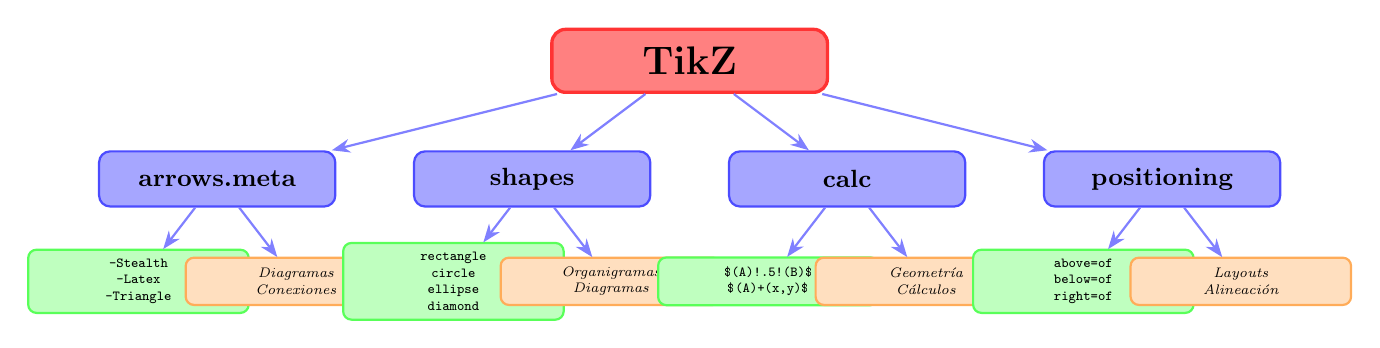
\begin{tikzpicture}[
		% Estilos de nodos
		root/.style={
			rectangle, rounded corners=5pt,
			fill=red!50, draw=red!80, very thick,
			minimum width=3.5cm, minimum height=0.8cm,
			font=\bfseries\Large
		},
		lib/.style={
			rectangle, rounded corners=4pt,
			fill=blue!35, draw=blue!70, thick,
			minimum width=3cm, minimum height=0.7cm,
			font=\bfseries\small
		},
		option/.style={
			rectangle, rounded corners=3pt,
			fill=green!25, draw=green!65,
			minimum width=2.8cm, minimum height=0.6cm,
			font=\tiny\ttfamily,
			align=center
		},
		app/.style={
			rectangle, rounded corners=3pt,
			fill=orange!25, draw=orange!65,
			minimum width=2.8cm, minimum height=0.6cm,
			font=\tiny\itshape,
			align=center
		},
		% Configuración del árbol vertical
		grow=down,
		level 1/.style={sibling distance=4cm, level distance=1.5cm},
		level 2/.style={sibling distance=2cm, level distance=1.3cm},
		level 3/.style={sibling distance=2cm, level distance=1.3cm},
		edge from parent/.style={draw, thick, -Stealth, blue!50}
		]
		
		\node[root] {TikZ}
		child {node[lib] {arrows.meta}
			child {node[option] {-Stealth\\-Latex\\-Triangle}}
			child {node[app] {Diagramas\\Conexiones}}
		}
		child {node[lib] {shapes}
			child {node[option] {rectangle\\circle\\ellipse\\diamond}}
			child {node[app] {Organigramas\\Diagramas}}
		}
		child {node[lib] {calc}
			child {node[option] {\$(A)!.5!(B)\$\\\$(A)+(x,y)\$}}
			child {node[app] {Geometría\\Cálculos}}
		}
		child {node[lib] {positioning}
			child {node[option] {above=of\\below=of\\right=of}}
			child {node[app] {Layouts\\Alineación}}
		};
		
	\end{tikzpicture}
\end{center}

\section*{Librería: groupplots}
\begin{center}
	\begin{tikzpicture}
		\begin{groupplot}[group style={group size=2 by 1, horizontal sep=2cm},
			width=5cm, height=4cm, grid=both]
			\nextgroupplot[title={$x^2$}]
			\addplot[blue, thick, domain=-2:2]{x^2};
			\nextgroupplot[title={$e^{-x}$}]
			\addplot[red, thick, domain=0:4]{exp(-x)};
		\end{groupplot}
	\end{tikzpicture}
\end{center}

\vspace{2cm}

\dirtree{%
	.1 TikZ Libraries/.
	.2 Flechas y conectores/.
	.3 arrows (clásica, obsoleta).
	.3 arrows.meta (sistema moderno de puntas de flecha).
	.3 bending (curvar flechas en trayectorias).
	.2 Posicionamiento y coordenadas/.
	.3 positioning (nodos relativos).
	.3 calc (cálculo de coordenadas).
	.3 quotes (etiquetas rápidas en caminos).
	.3 through (circunferencias/figuras que pasan por un punto).
	.2 Formas de nodos/.
	.3 shapes (colección general).
	.3 shapes.geometric (triángulo, rombo, trapecio).
	.3 shapes.misc (nube, estrella).
	.3 shapes.symbols (símbolos decorativos).
	.3 shapes.multipart (nodos con varias partes).
	.2 Estilos de relleno y trazos/.
	.3 patterns (patrones básicos).
	.3 patterns.meta (sistema moderno de patrones).
	.3 fadings (desvanecimientos).
	.3 shadings (degradados).
	.3 shadows, shadows.blur, shadows.shadow (sombras).
	.2 Capas y fondos/.
	.3 backgrounds (capas de fondo).
	.3 fit (nodos contenedores).
	.3 matrix (matriz de nodos).
	.2 Decoraciones/.
	.3 decorations.pathmorphing (zigzag, serpenteo, pasos aleatorios).
	.3 decorations.markings (marcas en trayectorias, flechas en mitad).
	.3 decorations.text (texto a lo largo de caminos).
	.3 decorations.fractals (fractales como curva de Koch).
	.3 decorations.footprints (huellas decorativas).
	.2 Grafos y árboles/.
	.3 trees (árboles jerárquicos).
	.3 graphs (sintaxis declarativa de grafos).
	.3 graphdrawing (algoritmos automáticos, requiere LuaLaTeX).
	.2 Geometría y matemáticas/.
	.3 angles (ángulos en figuras).
	.3 intersections (cálculo de intersecciones).
	.3 lindenmayersystems (fractales tipo plantas).
	.2 Extras/.
	.3 mindmap (mapas mentales).
	.3 calendar (calendarios).
	.3 plotmarks (marcadores de gráficas).
	.3 external (externalizar figuras en PDFs).
	.3 3d (soporte 3D básico).
} 

\vspace{1cm}

\dirtree{%
	.1 PGFPlots — Librerías y opciones/.
	.2 groupplots/.
	.3 Claves: {group style=\{group size=<c> by <r>, horizontal sep=<d>, vertical sep=<d>\}}.
	.3 Extras: {xticklabels at=edge bottom}, {yticklabels at=edge left}, {shared axis}.
	.3 Uso: paneles de subgráficas alineadas (comparativas).
	.2 fillbetween/.
	.3 Claves: {name path=<A/B>}, {fill between[of=A and B]}, {soft clip=\{domain=a:b\}}.
	.3 Variantes: {split}, {intersection segments}.
	.3 Uso: rellenar área entre dos curvas o en subintervalos.
	.2 statistics/.
	.3 Histograma: {ybar interval}, {hist=\{bins=<n>, density, data min=<v>, data max=<v>\}}.
	.3 Boxplot: {boxplot}, {boxplot/draw direction=y}, {table}.
	.3 Otros: {scatter src}, {error bars/.cd, y dir=both, y explicit}.
	.3 Uso: distribuciones, resúmenes estadísticos y datos con barras de error.
	.2 dateplot/.
	.3 Claves: {date coordinates in=x} (o y), {xticklabel=\textbackslash year-\textbackslash month-\textbackslash day}.
	.3 Filtros: {x filter/.code=\{...\}} para transformar fechas/formatos.
	.3 Uso: series temporales con eje de fechas.
	.2 colormaps/.
	.3 Claves: {colormap name=viridis} (hot, jet, plasma, magma, turbo...).
	.3 Meta: {point meta=...}, {mesh/cols=<n>, mesh/rows=<n>}.
	.3 Uso: superficies, mapas de calor con escalas perceptuales.
	.2 colorbrewer/.
	.3 Claves: {cycle list/Set2}, {cycle list/Paired}, {cycle list name=<paleta>}.
	.3 Uso: colores consistentes para múltiples series (categorías).
	.2 polar/.
	.3 Entorno: {polaraxis}.
	.3 Claves: {xtick=\{0,30,...,330\}}, {ytick distance=<d>}, {grid=both}.
	.3 Uso: gráficos en coordenadas polares (rosas, radar básico).
	.2 patchplots/.
	.3 Claves: {patch}, {patch type=triangle|rectangle}, {patch refines=<n>}.
	.3 Datos: mallas no regulares (FEM/CFD), {mesh/ordering=rowwise|colwise}.
	.3 Uso: superficies por parches triangulares/cuadriláteros.
	.2 ternary/.
	.3 Entorno: {ternaryaxis}.
	.3 Claves: {ternary limits relative}, {xlabel=\{\$A\$\}}, {ylabel=\{\$B\$\}}, {zlabel=\{\$C\$\}}.
	.3 Uso: composiciones que suman 1 o 100\% (geología/química).
	.2 smithchart/.
	.3 Entorno: {smithchart}.
	.3 Claves: {grid=both}, estilos de curvas de impedancia/reflexión, ticks especializados.
	.3 Uso: ingeniería RF (diagramas de Smith).
	.2 units/.
	.3 Integración: etiquetas con unidades (opcional siunitx).
	.3 Claves: {unit x label=<unidad>}, {unit y label=<unidad>}, {x SI prefix kilo}.
	.3 Uso: ejes con unidades y prefijos automáticos.
} 


\section*{Librería: patchplots}
\begin{center}
	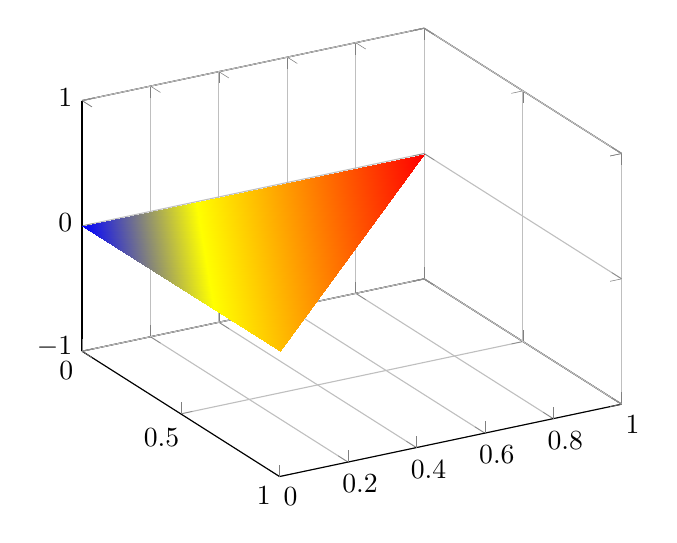
\begin{tikzpicture}
		\begin{axis}[view={60}{30}, grid=both]
			\addplot3[
			patch,
			patch type=triangle,
			shader=interp,
			point meta=\thisrow{c}
			] table {
				x y z c
				0 0 0 0
				1 0 0 1
				0 1 0 2
			};
		\end{axis}
	\end{tikzpicture}
\end{center}

\vspace{5mm}

% Comentar una sección completa:
\begin{comment}
	Este texto largo con fórmulas $x^2$, 
	tablas, figuras, etc. será completamente 
	ignorado durante la compilación.
\end{comment}

% Comentarios condicionales:
\includecomment{notas}  % o \excludecomment{notas}

\begin{notas}
	
	Contenido que aparece o desaparece según configuración
	
	\begin{verbatim}
		\usepackage{graphicx}
		\usepackage[dvipsnames]{xcolor} % u otra opción
		\usepackage{float}
		\usepackage{subcaption}
		\usepackage{tikz}
		\usetikzlibrary{3d}
		\usetikzlibrary{babel, patterns, patterns.meta, arrows.meta, calc, positioning, shapes.geometric, shapes.misc, shapes.symbols, fadings, shadings, shadows, backgrounds}
		\usetikzlibrary{backgrounds}
		\tikzset{help lines/.style={very thin, draw=gray!30}}
		contenidos...
	\end{verbatim}
\end{notas}

\begin{verbatim}
	\usepackage{graphicx}
	\usepackage[dvipsnames]{xcolor} % u otra opción
	\usepackage{float}
	\usepackage{subcaption}
	\usepackage{tikz}
	\usetikzlibrary{3d}
	\usetikzlibrary{babel, patterns, patterns.meta, arrows.meta, calc, positioning, shapes.geometric, shapes.misc, shapes.symbols, fadings, shadings, shadows, backgrounds}
	\usetikzlibrary{backgrounds}
	\tikzset{help lines/.style={very thin, draw=gray!30}}
	contenidos...
\end{verbatim}